%% ****** Start of file apstemplate.tex ****** %
%%
%%
%%   This file is part of the APS files in the REVTeX 4.2 distribution.
%%   Version 4.2a of REVTeX, January, 2015
%%
%%
%%   Copyright (c) 2015 The American Physical Society.
%%
%%   See the REVTeX 4 README file for restrictions and more information.
%%
%
% This is a template for producing manuscripts for use with REVTEX 4.2
% Copy this file to another name and then work on that file.
% That way, you always have this original template file to use.
%
% Group addresses by affiliation; use superscriptaddress for long
% author lists, or if there are many overlapping affiliations.
% For Phys. Rev. appearance, change preprint to twocolumn.
% Choose pra, prb, prc, prd, pre, prl, prstab, prstper, or rmp for journal
%  Add 'draft' option to mark overfull boxes with black boxes
%  Add 'showkeys' option to make keywords appear
%\documentclass[aps,prd,preprint,amsmath,amssymb,groupedaddress]{revtex4-2}
\documentclass[aps,prd,twocolumn,amsmath,amssymb,groupedaddress]{revtex4-2}
%\documentclass[aps,prl,preprint,superscriptaddress]{revtex4-2}
%\documentclass[aps,prl,reprint,groupedaddress]{revtex4-2}
\usepackage{graphicx}

% You should use BibTeX and apsrev.bst for references
% Choosing a journal automatically selects the correct APS
% BibTeX style file (bst file), so only uncomment the line
% below if necessary.
%\bibliographystyle{apsrev4-2}

\begin{document}

% Use the \preprint command to place your local institutional report
% number in the upper righthand corner of the title page in preprint mode.
% Multiple \preprint commands are allowed.
% Use the 'preprintnumbers' class option to override journal defaults
% to display numbers if necessary
%\preprint{}

%Title of paper
\title{Collision}

% repeat the \author .. \affiliation  etc. as needed
% \email, \thanks, \homepage, \altaffiliation all apply to the current
% author. Explanatory text should go in the []'s, actual e-mail
% address or url should go in the {}'s for \email and \homepage.
% Please use the appropriate macro foreach each type of information

% \affiliation command applies to all authors since the last
% \affiliation command. The \affiliation command should follow the
% other information
% \affiliation can be followed by \email, \homepage, \thanks as well.
\author{YU-CHIA LIN}
\email[]{yuchialin@arizona.edu}
%\homepage[]{Your web page}
%\thanks{}
%\altaffiliation{}
\affiliation{Department of Physics \& Astronomy, University of New Mexicoo, Albuquerque, New Mexico 87131, USA}
\affiliation{Department of Astronomy, University of Arizona, Tucson, Arizona 85721, USA}
\affiliation{Department of Physics, University of Arizona, Tucson, Arizona 85721, USA}
%Collaboration name if desired (requires use of superscriptaddress
%option in \documentclass). \noaffiliation is required (may also be
%used with the \author command).
%\collaboration can be followed by \email, \homepage, \thanks as well.
%\collaboration{}
%\noaffiliation

\date{\today}

\begin{abstract}
% insert abstract here
It has been a long-standing mystery how collisions and collective neutrino oscillations interact. We focus on one type of collision-generated instabilities as we investigate the impact of the collision term in neutrino flavor oscillations. In this model, the instability that may be common inside supernovae is caused by an asymmetry in the collisional interactions between neutrinos and antineutrinos. By creating analytical solutions, we sought to gain insight into such a mechanism. 

Additionally, our analytical approach demonstrates precisely when the exponential growth brought on by this instability begins, how quickly it increases, and how different factors affect the bump, making it potentially meaningful to a wider variety of collision-generated instabilities models.
\end{abstract}

% insert suggested keywords - APS authors don't need to do this
%\keywords{}
%\maketitle must follow title, authors, abstract, and keywords
\maketitle

% body of paper here - Use proper section commands
% References should be done using the \cite, \ref, and \label commands
\section{\label{sec:intro} INTRODUCTION}

\subsection{}
\subsubsection{}

\section{\label{sec:model} MODEL}
In this work, we consider the isotropic and homogeneous two-flavor neutrino flavor oscillation between $\nu_e$ and $\nu_\tau$, where $\nu_\tau$ represents a linear combination of the physical $\mu$ and $\tau$ flavor neutrino.

Denoting the neutrino flavor density matrix and the corresponding polarization vector as
\begin{equation}
	\rho = \begin{bmatrix}
		\rho_{11} ~~~ \rho_{12} \\
		\rho_{21} ~~~ \rho_{22}
	\end{bmatrix}
\end{equation}
and $\textbf{P}$ respectively, or
\begin{eqnarray}
	\rho_{ex} &\equiv& \rho_{21} = \frac{1}{2}\left(P_x + i P_y\right) \\
    \rho &=& \frac{1}{2} \left(P_0+\textbf{P} \cdot \sigma\right)
\end{eqnarray}, where $P_i$ is the $i$ component of $\textbf{P}$. 

As for the collision processes(P), we consider three types processes, absorption and emission (AE), charged current
scattering (CC), and neutral-current scattering (NC). The corresponding polarization vectors in equilibrium states and  are denoted as $\textbf{P}^{P}$ and $P_0^P$. Also, the corresponding coefficients for each process are $\Gamma_{P} = diag \left(\Gamma^{P}_e/2, ~\Gamma^{P}_x/2 \right)$, and we could define $\Gamma^{P}_\pm = \left(\Gamma^{P}_e \pm  \Gamma^{P}_x\right)/2$.

There are the same parameters for antineutrinos, and the bar cap is added to indicate. Then, we could write down the equations of motion for polarization vectors as follows (see Ref.~[\onlinecite{2021arXiv210411369J}]):
\begin{widetext}
\begin{eqnarray} 
	\dot{\textbf{P}} &=& \omega \textbf{B} \times \textbf{P}+ \mu (\textbf{P}-\bar{\textbf{P}}) \times \textbf{P} - \Gamma^{CC}_+ \textbf{P}_T + \Gamma^{AE}_+ (\textbf{P}^{AE} - \textbf{P}) + \Gamma^{AE}_- (P^{AE}_0 -P_0)\textbf{z} \\
	\dot{\bar{\textbf{P}}} &=& -\omega \textbf{B} \times \bar{\textbf{P}}+ \mu (\textbf{P}-\bar{\textbf{P}}) \times \bar{\textbf{P}} - \bar{\Gamma}^{CC}_+ \bar{\textbf{P}}_T + \bar{\Gamma}^{AE}_+ (\bar{\textbf{P}}^{AE} - \bar{\textbf{P}}) + \bar{\Gamma}^{AE}_- (\bar{P}^{AE}_0 -\bar{P}_0)\textbf{z} \\
	\dot{P_0} &=& \Gamma^{AE}_+ (P^{AE}_0 -P_0) + \Gamma^{AE}_- (P^{AE}_z -P_z) \\
	\dot{\bar{P_0}} &=& \bar{\Gamma}^{AE}_+ (\bar{P}^{AE}_0 -\bar{P}_0) + \bar{\Gamma}^{AE}_- (\bar{P}^{AE}_z -\bar{P}_z)
\end{eqnarray}
\end{widetext}
, where angular frequency in vacuum $\omega = \frac{\delta m^2}{2E}$ and $\mu = \sqrt{2} G_F$.

In the following calculations, unless otherwise specified, we choose the following parameter values
\begin{eqnarray}
	\label{equ:par_constant}
	\begin{bmatrix}
		\omega \\ 
		\mu \\ 
		\theta\\
		\textbf{B}
	\end{bmatrix}
	= \begin{bmatrix}
		0.3 ~km^{-1} \\ 
		6 \times 10^5 ~km^{-1} \\ 
		10^{-6} \\
		-sin 2\theta~\textbf{e}_x^f + cos 2\theta~\textbf{e}_z^f 
	\end{bmatrix}
\end{eqnarray}
\begin{eqnarray}
	\label{equ:par_gamma}
	\begin{bmatrix}
		\Gamma^{CC}_+ \\ \Gamma^{AE}_+ \\ \Gamma^{AE}_-
	\end{bmatrix}
	= \begin{bmatrix}
		0.5/11.4 ~km^{-1} \\ 0.5/0.417 ~km^{-1} \\ 0.5/0.417 ~km^{-1}
	\end{bmatrix}
\end{eqnarray}

\begin{eqnarray}
	\label{equ:par_bgamma}
	\begin{bmatrix}
		\bar{\Gamma}^{CC}_+ \\ \bar{\Gamma}^{AE}_+ \\ \bar{\Gamma}^{AE}_-
	\end{bmatrix}
	= \begin{bmatrix}
		0.5/37.2 ~km^{-1} \\ 0.5/4.36 ~km^{-1} \\ 0.5/4.36 ~km^{-1} 
	\end{bmatrix}
\end{eqnarray}

\begin{eqnarray}
	\label{equ:par_P}
	\begin{bmatrix}
		\textbf{P}^{AE} \\ P^{AE}_0 \\ \bar{\textbf{P}}^{AE} \\ \bar{P}^{AE}_0
	\end{bmatrix}
	= \begin{bmatrix}
		2 ~\textbf{e}_z^f\\ 4 \\ 1.5 ~\textbf{e}_z^f \\ 3.5
	\end{bmatrix}
\end{eqnarray}

Also, the initial condition
\begin{eqnarray}
	\label{equ:ini_condition}
	\begin{bmatrix}
		\textbf{P} \\ P_0 \\ \bar{\textbf{P}} \\ \bar{P}_0
	\end{bmatrix}
	= \begin{bmatrix}
		2 ~\textbf{e}_z^f\\ 4 \\ 1.5 ~\textbf{e}_z^f \\ 3.5
	\end{bmatrix}
\end{eqnarray}

Note that we use $10^{33} ~cm^{-3}$ as the unit length in the vector space of polarization vectors.

\section{\label{sec:results} Results}
Here we will try to solve the equations of motion in the linear region and compare the analytical results with the numerical results. With this analytical solution, we could find an approximate expression for the start time and the growth rate of exponential growth in the limit cases, which characterize the bump.

\subsection{\label{subsec:num} Numerical Solution}
Given initial conditions and parameters as described in equation (\ref{equ:par_constant}), (\ref{equ:par_gamma}), (\ref{equ:par_bgamma}), (\ref{equ:par_P}), and (\ref{equ:ini_condition}), we could obtain the numerical solutions via the equations of motion of polarization vectors. We plot the results in FIG. \ref{fig:compare_rho} and show them as solid lines.

It should be emphasized that there is a requirement for the precision of numerical simulations in order to produce consistent results. We need to be quite careful, especially when $\mu$ are really large or $\theta$ is quite little. The detailed reasoning behind it will be discussed in subsection \ref{subsec:precision_of_num}.

\subsection{\label{subsec:linear} Linearlized Equations of Motion}
We need to determine when the equations of motion is a system of linear equations in order to obtain an analytical solution.
Actually, when $P_x, ~P_y \ll P_z \sim 1$, the equations of motion become

\begin{widetext}
\begin{eqnarray}
	i \partial_t \rho_{ex} = \omega ~sin2\theta P_{z}
	+\left[-\omega ~cos2\theta-\sqrt{2}G_F(n_{\bar{\nu}_e}-n_{\bar{\nu}_x})- i \Gamma \right]\rho_{ex} + \sqrt{2}G_F(n_{\nu_e}-n_{\nu_x}) \bar{\rho}_{ex}\\
	i \partial_t \bar{\rho}_{ex} = - \omega ~sin2\theta \bar{P}_{z} +\left[+\omega ~cos2\theta + \sqrt{2}G_F(n_{\nu_e}-n_{\nu_x}) - i \bar{\Gamma} \right]\bar{\rho}_{ex} -\sqrt{2}G_F(n_{\bar{\nu}_e}-n_{\bar{\nu}_x}) \rho_{ex}
\end{eqnarray}
\end{widetext}
,
where
\begin{equation}
\begin{cases}
	\Gamma \equiv \Gamma^{AE} + \Gamma^{CC}
	\\
	\bar{\Gamma} \equiv \bar{\Gamma}^{AE} + \bar{\Gamma}^{CC}
\end{cases}
\end{equation}

Let
\begin{equation}
\begin{cases}
	\mu_+ \equiv \left(\frac{S+D}{2}\right) \mu
	\\
	\mu_- \equiv \left(\frac{S-D}{2}\right) \mu
\end{cases}
\end{equation}
, 
\begin{equation}
	\begin{cases}
		S \equiv |\vec{S}(0)| =  n_{\nu_e} - n_{\nu_x} + n_{\bar{\nu}_e} - n_{\bar{\nu}_x}
		\\
		D \equiv |\vec{D}(0)| =  n_{\nu_e} - n_{\nu_x} - n_{\bar{\nu}_e} + n_{\bar{\nu}_x}
	\end{cases}
\end{equation}, 
and
\begin{equation}
A = \begin{bmatrix}
	-\omega ~cos2\theta-\mu_--i\Gamma ~~~~~~~~~ \mu_+ ~~~~~~~~~~~~~~~~\\ ~~~~~~~~~ -\mu_- ~~~~~~~~ \omega ~cos2\theta+\mu_+-i\bar{\Gamma}
\end{bmatrix}
\end{equation}

, we have
\begin{equation}
	\label{equ:EOM_matrix}
	i \partial_t \begin{bmatrix}
		\rho_{ex} \\ \bar{\rho}_{ex}
	\end{bmatrix} =
	\begin{bmatrix}
		\omega ~sin2\theta \\ - \omega ~sin2\theta
	\end{bmatrix} + A \begin{bmatrix}
		\rho_{ex} \\ \bar{\rho}_{ex}
	\end{bmatrix}
\end{equation}

Notice that, $P_{z}$ and $\bar{P}_{z}$ are both close to 1 under this limitation condition.

\subsection{\label{subsec:analytic} Analytic Solution}
\begin{figure*}[t]
	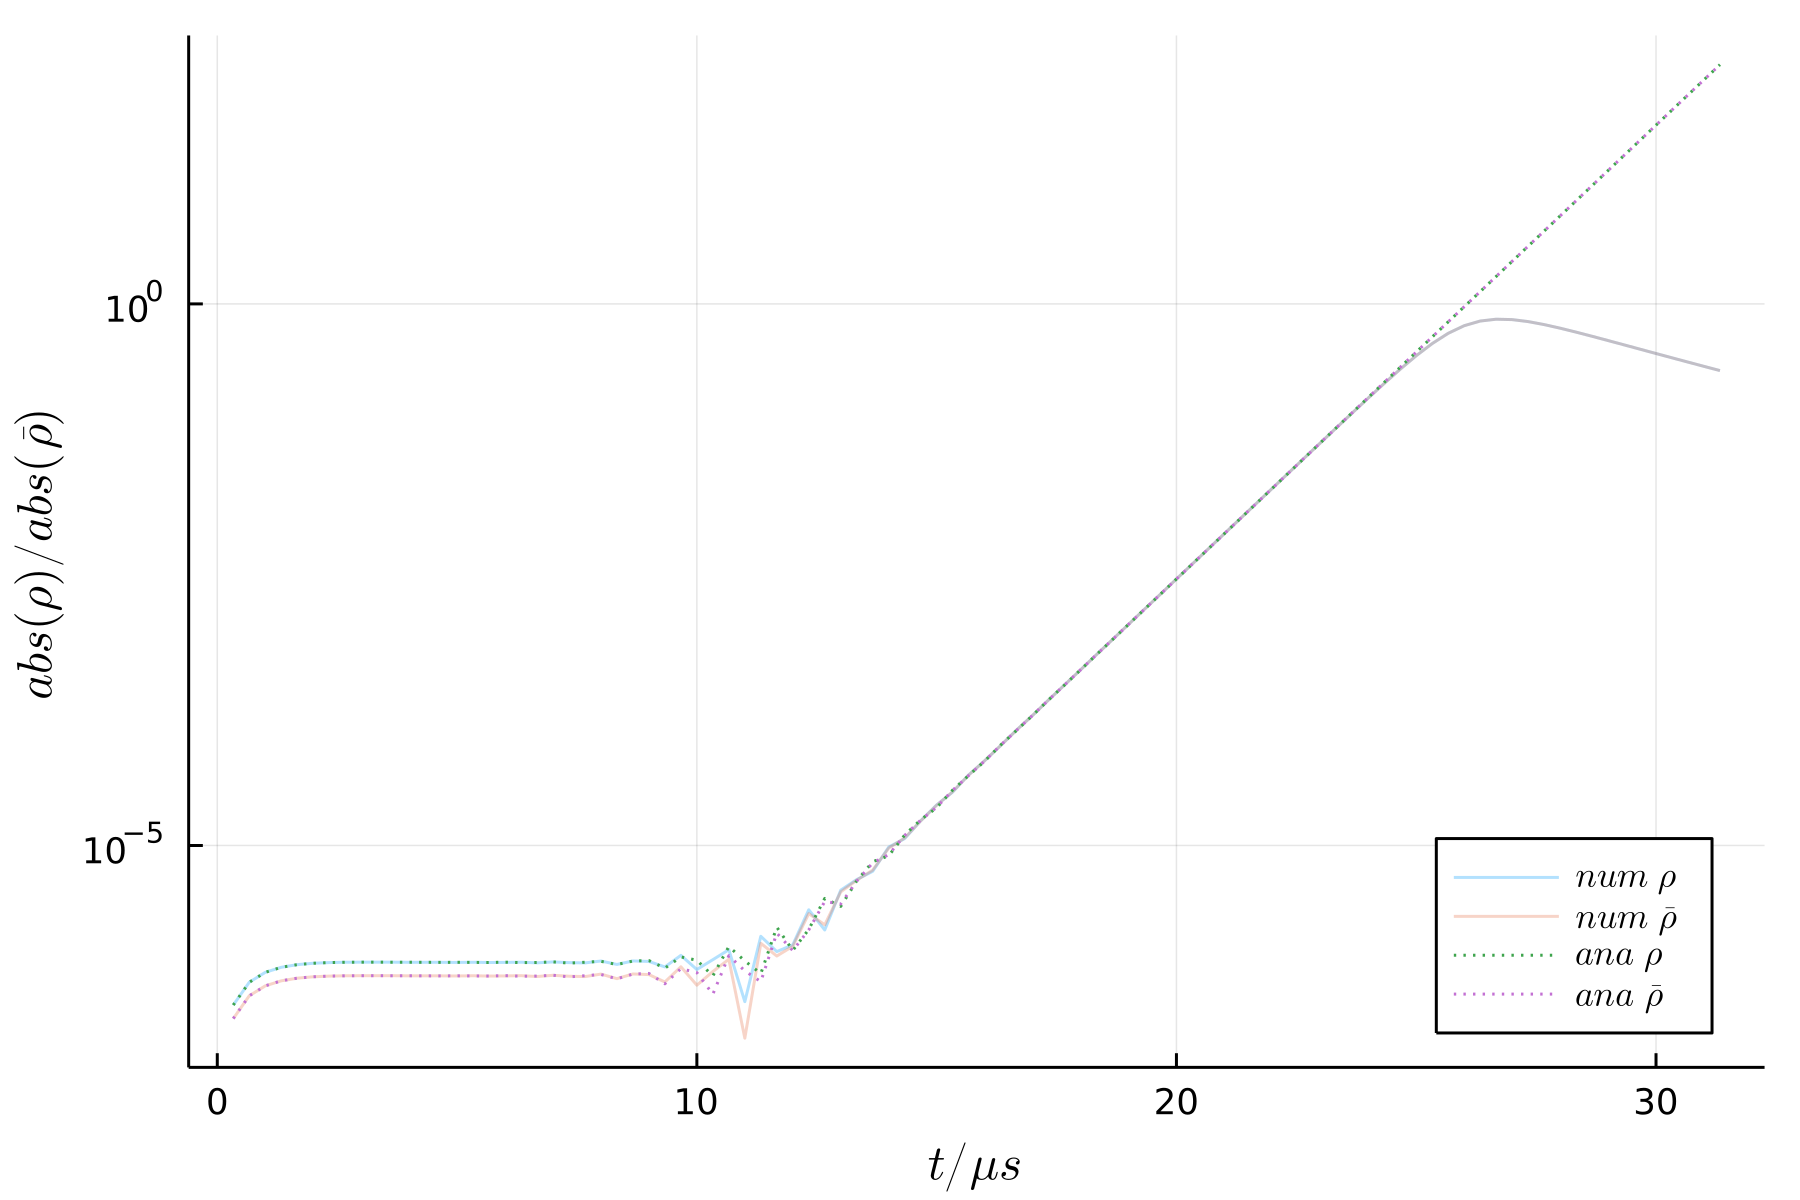
\includegraphics[scale=0.28]{compare_rho.png}
	\caption{\label{fig:compare_rho} The absolute value of $\rho_{ex}$ and $\bar{\rho}_{ex}$ over time}
\end{figure*}

Assume
\begin{equation}
	\begin{cases}
		\rho_{ex}(t) = \rho^0_{ex} + Q e^{-i\Omega t}
		\\
		\bar{\rho}_{ex}(t) = \bar{\rho}^0_{ex} + \bar{Q} e^{-i\Omega t}
	\end{cases}
\end{equation}
from equation (\ref{equ:EOM_matrix}), we then have
\begin{eqnarray}
	\label{equ:eigenfunction}
	\Omega 
	\begin{bmatrix}
		Q \\ \bar{Q}
	\end{bmatrix}
	= A
	\begin{bmatrix}
		Q \\ \bar{Q}
	\end{bmatrix}
\end{eqnarray}, where $\rho^0_{ex}$ and $\bar{\rho}^0_{ex}$ satisfy
\begin{equation}
	\label{equ:rho0}
	0= \begin{bmatrix}
		\omega ~sin2\theta \\ - \omega ~sin2\theta
	\end{bmatrix}  + 
	A \begin{bmatrix} \rho^0_{ex} \\ \bar{\rho}^0_{ex}
	\end{bmatrix}
\end{equation}

Therefore, we could solve the eigenvalue problem of matrix $A$, and denote the eigenvalues and normalized eigenvectors as $\Omega_\pm$ and $\vec{v}_\pm$ respectively.

Then,
\begin{eqnarray}
\label{equ:rho_ana}
\begin{bmatrix}
	\rho_{ex} (t)\\ \bar{\rho}_{ex} (t)
\end{bmatrix}
&=& \begin{bmatrix} 
	\rho^0_{ex} \\ \bar{\rho}^0_{ex}
\end{bmatrix} + 
Q_+ \vec{v}_+
e^{-i \Omega_{+} \bf{t}} +
Q_- \vec{v}_-
e^{-i \Omega_{-} \bf{t}} \nonumber \\
&=&
v
\begin{bmatrix}
	Q_-e^{-i \Omega_{-} \bf{t}} \\ Q_+e^{-i \Omega_{+} ~\bf{t}}
\end{bmatrix} + 
\begin{bmatrix} 
	\rho^0_{ex} \\ \bar{\rho}^0_{ex}
\end{bmatrix}
\end{eqnarray}
, where 
\begin{eqnarray}
v \equiv
\begin{bmatrix}
	\vec{v}_- ~~ \vec{v}_+
\end{bmatrix}
\end{eqnarray}
and $Q_+$ and $Q_-$ satisfy
\begin{eqnarray}
\label{equ:Q}
\begin{bmatrix}
	Q_- \\ Q_+
\end{bmatrix} =
v^{-1}
\begin{bmatrix}
	- \rho^0_{ex} \\ -\bar{\rho}^0_{ex}
\end{bmatrix}
\end{eqnarray}

Now, we could compare this analytical solution with the numerical solution in FIG. \ref{fig:compare_rho}.


\subsection{\label{subsec:approximation} Approximate and Analytical Expressions}

\begin{figure}[b]
	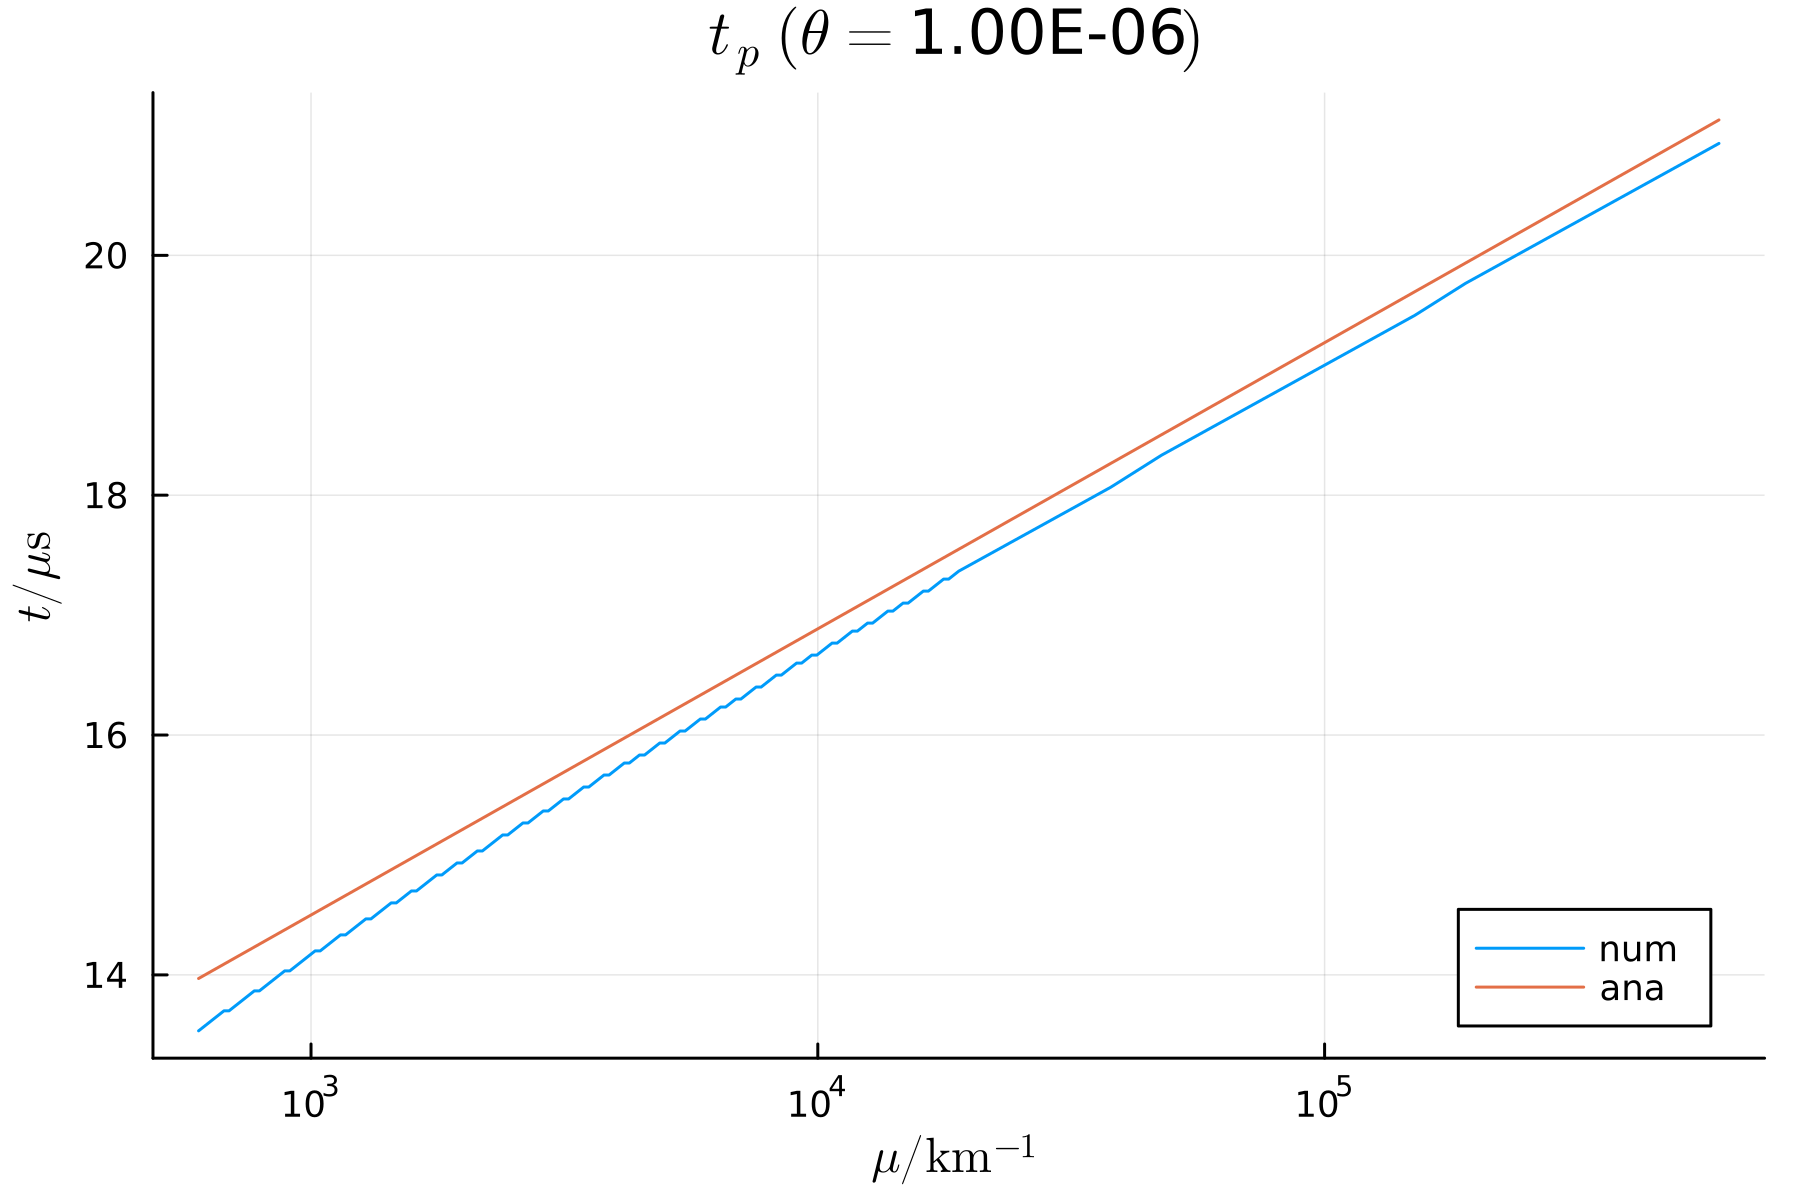
\includegraphics[scale=0.13]{compare_tp_mu.png}
	\caption{\label{fig:compare_tp_mu} Comparing $t_p$ in equation (\ref{equ:tp}) with numerical simulation for different $\mu$}
\end{figure}
\begin{figure}[b]
	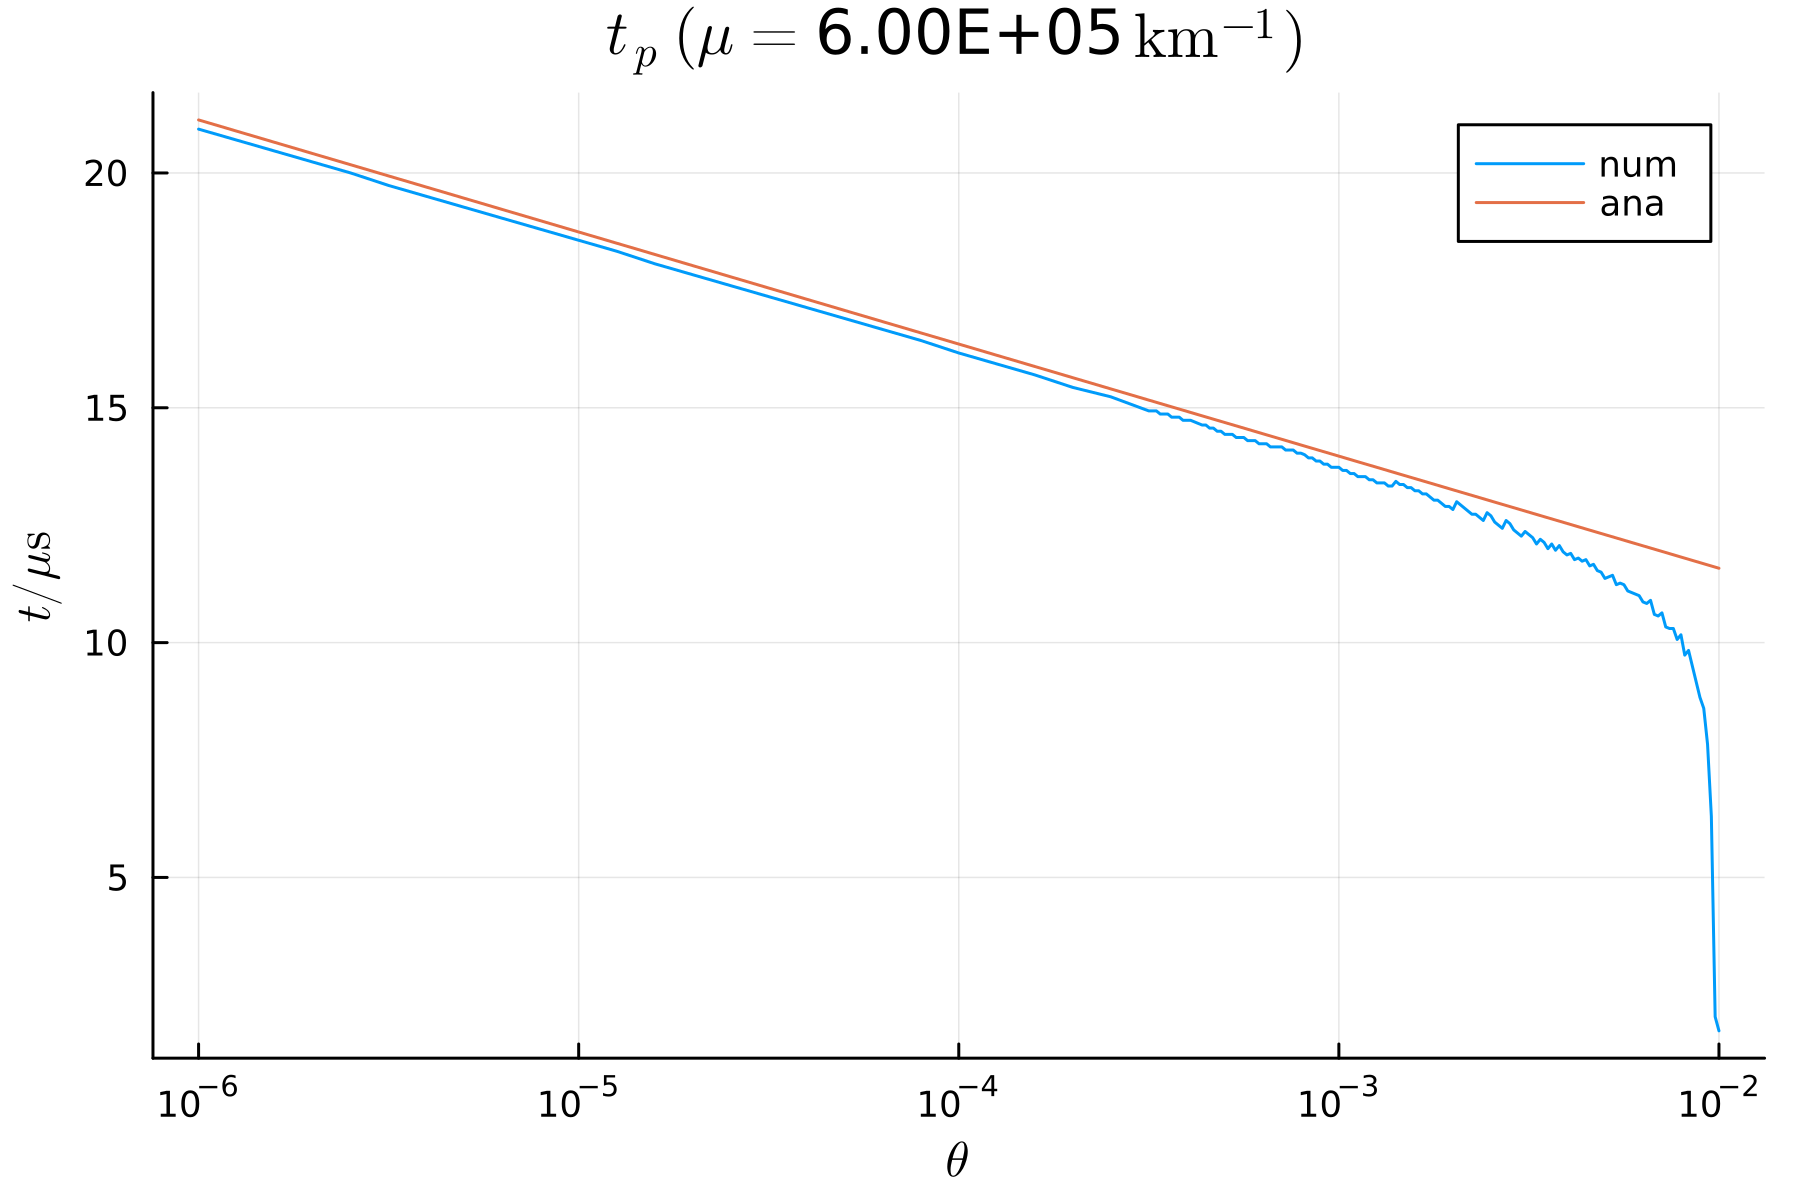
\includegraphics[scale=0.13]{compare_tp_theta.png}
	\caption{\label{fig:compare_tp_theta} Comparing $t_p$ in equation (\ref{equ:tp}) with numerical simulation for different $\theta$}
\end{figure}

In this subsection, we consider $\mu S, ~\mu D \gg \omega, ~\Gamma, ~\bar{\Gamma} $ and $\theta \ll 1$. Then, the zero order approximation of equation (\ref{equ:rho0}) 
\begin{eqnarray}
	\begin{bmatrix} 
		\rho^0_{ex} \\ \bar{\rho}^0_{ex}
	\end{bmatrix} 
	&=& A^{-1} 
	\begin{bmatrix}
		-\omega ~sin2\theta \\ + \omega ~sin2\theta
	\end{bmatrix} \nonumber \\
	\label{equ:0_rho0}
	&\simeq&
	\frac{2\omega \theta}{\omega S + i\left[(S+D) \Gamma + (D-S) \bar{\Gamma}\right]}
	\begin{bmatrix}
		S+D \\ S-D
	\end{bmatrix} \\
	&\sim& \theta^1 \mu^0
\end{eqnarray}

On the other hand, the eigenvalues of A is
\begin{eqnarray}
	\begin{bmatrix}
		\Omega_+ \\ \Omega_-
	\end{bmatrix} \simeq
	\begin{bmatrix}
		\mu D + i \left[\frac{S}{2D}\left(\Gamma-\bar{\Gamma}\right)-\frac{1}{2}\left(\Gamma+\bar{\Gamma}\right)\right]\\
		\frac{\omega S}{D} - i \left[\frac{S}{2D}\left(\Gamma-\bar{\Gamma}\right)+\frac{1}{2}\left(\Gamma+\bar{\Gamma}\right)\right]
	\end{bmatrix}
\end{eqnarray}
Then, we could get the zero order approximation of the eigenvectors matrix 
\begin{eqnarray}
	\label{equ:0_eigenvectors}
	v \simeq
	\begin{bmatrix}
		\frac{S+D}{\sqrt{2}\sqrt{S^2+D^2}} ~~~~~ \frac{1}{\sqrt{2}}\\
		\frac{S-D}{\sqrt{2}\sqrt{S^2+D^2}} ~~~~~ \frac{1}{\sqrt{2}}
	\end{bmatrix}
\end{eqnarray}, or
\begin{eqnarray}
	\label{equ:0_antieigenvectors}
	v^{-1}\simeq
	\begin{bmatrix}
		\frac{\sqrt{S^2+D^2}}{\sqrt{2}D} ~~~ -\frac{\sqrt{S^2+D^2}}{\sqrt{2}D}\\
		\frac{D-S}{\sqrt{2}D} ~~~~~~~~~~ \frac{D+S}{\sqrt{2}D}
	\end{bmatrix}
\end{eqnarray}

Substituting equation (\ref{equ:0_rho0}) and equation (\ref{equ:0_antieigenvectors}) into equation (\ref{equ:Q}), the zero order approximation of Q:
\begin{eqnarray}
	\label{equ:0_Q}
	\begin{bmatrix}
		Q_- \\ Q_+
	\end{bmatrix} \simeq \frac{-4\sqrt{2}\omega \theta \sqrt{S^2+D^2}}{\omega S + i\left[(S+D) \Gamma + (D-S) \bar{\Gamma}\right]}
	\begin{bmatrix}
	1 \\ 0
	\end{bmatrix}
\end{eqnarray}
Here we discover that the zeroth order of $Q_+$ is approximately zero, explaining why the exponential growth takes some time to start,  why a high level of precision is necessary for the numerical solution to produce an accurate bump (see subsection \ref{subsec:precision_of_num}).

When $|\rm{Im}\{\Omega_-\}| t>>1$, equation (\ref{equ:rho_ana}) could be simplified to
\begin{eqnarray}
	\begin{bmatrix}
		\rho_{ex} (t)\\ \bar{\rho}_{ex} (t)
	\end{bmatrix}
	\simeq
	Q_+e^{-i \Omega_{+} ~\bf{t}}
	\begin{bmatrix}
		v_{12}  \\ v_{22}
	\end{bmatrix} + 
	\begin{bmatrix} 
		\rho^0_{ex} \\ \bar{\rho}^0_{ex}
	\end{bmatrix}
\end{eqnarray}

Therefore, to get the start time of the exponential growing, we have to find the first order nonzero approximation of $Q_+$:
\begin{eqnarray}
	\label{equ:Qp}
	Q_+	&\simeq&
	\frac{-2\sqrt{2}\omega \theta}{\mu \omega S - i \left[\mu_+ \Gamma - \mu_- \bar{\Gamma} \right]}
	\begin{bmatrix}
		-\frac{\mu_-'}{\mu D} \\ \frac{\mu_+}{\mu D}
	\end{bmatrix}^T
	\begin{bmatrix}
		2\mu_+ + \omega - i \bar{\Gamma} \\ 2\mu_- + \omega + i \Gamma
	\end{bmatrix} \nonumber \\
	&\simeq&
	\frac{-2 \theta\omega S}{\mu D^2}\\
	&\sim&
	\theta^1 \mu^{-1}
\end{eqnarray}, where $\mu_-' \equiv \mu_- + \omega + i \Gamma + \Omega_-$.

Finally, we could obtain the start time of the exponential growth
\begin{eqnarray}
	t_s	&\simeq& 
	\frac{1}{\rm{Im}\{\Omega_+\}}ln(\frac{\left| \left(\rho^0_{ex}, ~\bar{\rho}^0_{ex}\right) \right|}{\left|Q_+\left(v_{12}, ~ v_{22}\right)\right|})	\nonumber \\
	&\simeq&
	\frac{1}{\left[\frac{S}{2D}\left(\Gamma-\bar{\Gamma}\right)-\frac{1}{2}\left(\Gamma+\bar{\Gamma}\right)\right]} \nonumber \\
	&&\ln(\frac{2\mu D^2\sqrt{S^2+D^2}}{S\sqrt{\omega^2S^2+\left[(S+D) \Gamma + (D-S) \bar{\Gamma}\right]^2}}) \\
	&\sim& \ln(\mu^1 \theta^0)
\end{eqnarray}
which is independent of $\theta$.

Moreover, with a similar analysis, we could get the time it takes for the absolute density, $\left| \left(\rho^0_{ex}, ~\bar{\rho}^0_{ex}\right) \right|$, to reach a particular density $(\rho_{p}) \ll 1$:
\begin{eqnarray}
	\label{equ:tp}
	t_{p}	&\simeq& 
	\frac{1}{\rm{Im}\{\Omega_+\}}ln(\frac{\rho_{p}}{\left|Q_+\left(v_{12}, ~ v_{22}\right)\right|})	\nonumber \\
	&\simeq&
	\frac{1}{\left[\frac{S}{2D}\left(\Gamma-\bar{\Gamma}\right)-\frac{1}{2}\left(\Gamma+\bar{\Gamma}\right)\right]} \ln(\frac{\rho_{p} \mu D^2}{2\theta \omega S}) \\
	&\sim& \ln(\mu^1 \theta^{-1})
\end{eqnarray}

For $\rho_p = 0.01$, we could compare the results of equation (\ref{equ:tp}) with the numerical simulation in FIG. \ref{fig:compare_tp_mu} and \ref{fig:compare_tp_theta}.

\section{\label{sec:disscussion} DISCUSSION}
In this section, we'll go into more detail about how analytical solutions give us detailed knowledge that will enable us to comprehend the complete model and the mechanism underlying collision-generated instabilities.

\subsection{\label{subsec:precision_of_num}Precision Requirements for Numerical Simulations}
Substituting the parameters into equation (\ref{equ:Qp}), we have 
\begin{eqnarray}
	\label{equ:Qp_num}
	\left|Q_+\right|
	&\simeq&
	\frac{2 \theta\omega S}{\mu D^2}\nonumber \\
	&\simeq&
	1.4 \times 10^{-11} \left(\frac{\theta}{10^{-6}}\right) \left(\frac{\mu}{6 \times 10^5 \rm{~km^{-1}}}\right)^{-1}
\end{eqnarray}
Therefore, to get a realistic and accurate bump shape, the numerical simulation precision should be much smaller than $Q_+$. 

\subsection{\label{subsec:deviation} Deviation between Analytical Solution and Numerical Simulation}

The deviation of the analytical solution derived from the linear system of equations and the numerical simulation steadily grows, as seen in FIG. \ref{fig:compare_tp_mu} and \ref{fig:compare_tp_theta}, as $\theta$ increases or $\mu$ decreases. This is because of the influence of nonlinear terms on numerical simulations.

\section{\label{sec:conclusion} CONCLUSIONS}

% If in two-column mode, this environment will change to single-column
% format so that long equations can be displayed. Use
% sparingly.
%\begin{widetext}
% put long equation here
%\end{widetext}

% figures should be put into the text as floats.
% Use the graphics or graphicx packages (distributed with LaTeX2e)
% and the \includegraphics macro defined in those packages.
% See the LaTeX Graphics Companion by Michel Goosens, Sebastian Rahtz,
% and Frank Mittelbach for instance.
%
% Here is an example of the general form of a figure:
% Fill in the caption in the braces of the \caption{} command. Put the label
% that you will use with \ref{} command in the braces of the \label{} command.
% Use the figure* environment if the figure should span across the
% entire page. There is no need to do explicit centering.

% \begin{figure}
% \includegraphics{}%
% \caption{\label{}}
% \end{figure}

% Surround figure environment with turnpage environment for landscape
% figure
% \begin{turnpage}
% \begin{figure}
% \includegraphics{}%
% \caption{\label{}}
% \end{figure}
% \end{turnpage}

% tables should appear as floats within the text
%
% Here is an example of the general form of a table:
% Fill in the caption in the braces of the \caption{} command. Put the label
% that you will use with \ref{} command in the braces of the \label{} command.
% Insert the column specifiers (l, r, c, d, etc.) in the empty braces of the
% \begin{tabular}{} command.
% The ruledtabular enviroment adds doubled rules to table and sets a
% reasonable default table settings.
% Use the table* environment to get a full-width table in two-column
% Add \usepackage{longtable} and the longtable (or longtable*}
% environment for nicely formatted long tables. Or use the the [H]
% placement option to break a long table (with less control than 
% in longtable).
% \begin{table}%[H] add [H] placement to break table across pages
% \caption{\label{}}
% \begin{ruledtabular}
% \begin{tabular}{}
% Lines of table here ending with \\
% \end{tabular}
% \end{ruledtabular}
% \end{table}

% Surround table environment with turnpage environment for landscape
% table
% \begin{turnpage}
% \begin{table}
% \caption{\label{}}
% \begin{ruledtabular}
% \begin{tabular}{}
% \end{tabular}
% \end{ruledtabular}
% \end{table}
% \end{turnpage}

% Specify following sections are appendices. Use \appendix* if there
% only one appendix.
%\appendix
%\section{}

% If you have acknowledgments, this puts in the proper section head.
%\begin{acknowledgments}
% put your acknowledgments here.
%\end{acknowledgments}

% Create the reference section using BibTeX:
\bibliography{Collision}

\end{document}
%
% ****** End of file apstemplate.tex ******

